%
%   Chapter Method
%
%   Qing-Cheng Li (r01922024 at csie dot ntu dot edu dot tw)
%   R.O.C.103.07
%
\chapter{研究方法}
\label{c:method}

本章節將介紹使用的資料集、欲偵測的實體特性及使用的方法與步驟。
本研究主要利用PATTY提供的關係釋義中包含的關係與樣式,
透過樣式有無出現在文句之中來判斷文件中是否具有某種關係。
以下小節將詳述之。

\section{特性偵測}
\subsection{以樣式偵測特性}
本研究將實體與實體間存在的關聯<實體甲, 關係, 實體乙>中的關係視為實體甲所具有的特性,
例如「賈伯斯於1955年出生於舊金山」包含了實體「賈伯斯」與「舊金山」,
在這個句子中,這兩個實體存在一組關聯<賈伯斯,出生於,舊金山>,
因此賈伯斯這個實體擁有「出生地」這樣的特性。
%本研究所欲偵測之實體特性其實是實體間的關係。    % ?

在上面這個例子之中,想要知道有沒有「出生地」這個特性,
可以透過「某人出生於某地」這樣的句子得知,
我們猜想,實體的特性應該有特定語句可以描述,
像是「出生地」這個特性就可透過「出生於」這樣的樣式來得知。

而PATTY正好提供了這樣的資源,如圖\ref{i:patty-online}。給定一個特性,
例如PATTY認為YAGO中的「wasBornIn」關係可以用「[[con]] grew up」、「was bron [[con]] grew up」等樣式來描述。

\begin{figure}
    \centering
    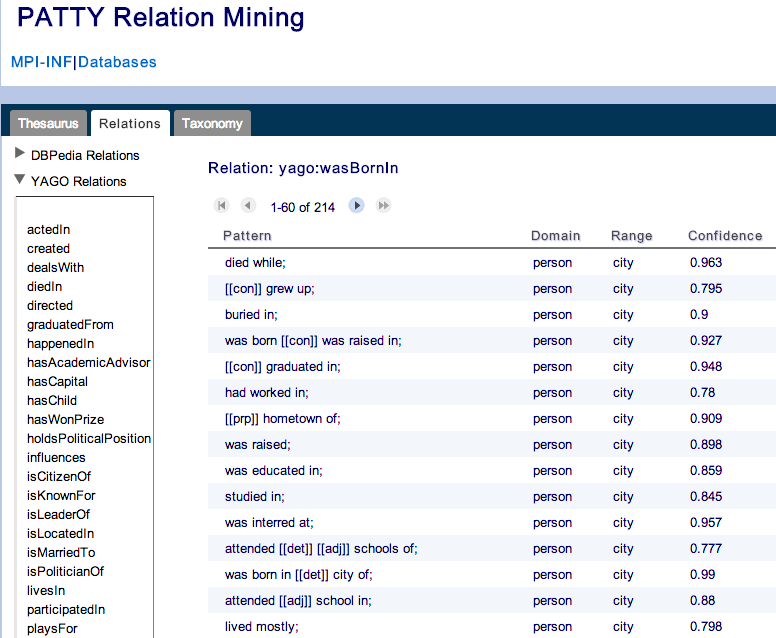
\includegraphics[width=0.5\textwidth]{images/03-patty-online}
    \caption{PATTY Online Relations}
    \label{i:patty-online}
\end{figure}

利用PATTY所提供的關係與樣式,本研究假設當在文句中看到一個樣式時,
該處便存在該樣式於PATTY中所屬的關係,亦即實體特性。
本研究將嘗試利用樣式來偵測表\ref{t:yago-relation}中的YAGO關係是否存在一份文件之中。

%t:yago-relation
\begin{table}[t]
    \begin{center}
        \footnotesize
        \begin{tabular}{|l||c|c|c|}
        \hline
        YAGO Relation & Domain & Range & Number of patterns \\
        \hline
        actedIn & wordnet\_actor & wordnet\_movie & 2023 \\
        created & yagoLegalActor & Thing & 3215 \\
        dealsWith & wordnet\_location & wordnet\_location & 366 \\
        diedIn & wordnet\_person & wordnet\_city & 1352 \\
        directed & wordnet\_person & wordnet\_movie & 1228 \\
        graduatedFrom & wordnet\_person & wordnet\_university & 2129 \\
        happenedIn & wordnet\_event & yagoGeoEntity & 47 \\
        hasAcademicAdvisor & wordnet\_person & wordnet\_person & 632 \\
        hasCapital & wordnet\_location & wordnet\_location & 24 \\
        hasChild & wordnet\_person & wordnet\_person & 3620 \\
        hasWonPrize & yagoLegalActorGeo & wordnet\_award & 78 \\
        holdsPoliticalPosition & wordnet\_person & wordnet\_person & 1173 \\
        influences & wordnet\_person & wordnet\_person & 2461 \\
        isCitizenOf & wordnet\_person & wordnet\_country & 813 \\
        isKnownFor & yagoLegalActor & Thing & 1574 \\
        isLeaderOf & wordnet\_person & yagoLegalActorGeo & 465 \\
        isLocatedIn & yagoPermanentlyLocatedEntity & yagoGeoEntity & 1300 \\
        isMarriedTo & wordnet\_person & wordnet\_person & 4276 \\
        isPoliticianOf & wordnet\_person & wiki\_states\_of\_US & 465 \\
        livesIn & wordnet\_person & wordnet\_location & 718 \\
        participatedIn & yagoLegalActorGeo & Thing & 89 \\
        playsFor & wordnet\_person & wordnet\_organization & 1491 \\
        wasBornIn & wordnet\_person & wordnet\_city & 1226 \\
        worksAt & wordnet\_person & wordnet\_organization & 1602 \\
        \hline
        \end{tabular}
        \caption{YAGO Relations in PATTY}
        \label{t:yago-relation}
    \end{center}
\end{table}


\subsection{偵測步驟}

本研究自內容串流的文件中偵測實體特性的偵測步驟主要可以分成兩大步驟 :
(1)樣式比對(Pattern Matching)與(2)特性篩選(Property Filtering)。

當一份文件出現時,偵測系統會先將

\section{樣式比對}

\section{特性篩選}

\section{}
\section{消除歧義}


